% Created 2018-04-02 lun 17:39
% Intended LaTeX compiler: pdflatex
\documentclass[xcolor={usenames,svgnames,dvipsnames}]{beamer}
\usepackage[utf8]{inputenc}
\usepackage[T1]{fontenc}
\usepackage{graphicx}
\usepackage{grffile}
\usepackage{longtable}
\usepackage{wrapfig}
\usepackage{rotating}
\usepackage[normalem]{ulem}
\usepackage{amsmath}
\usepackage{textcomp}
\usepackage{amssymb}
\usepackage{capt-of}
\usepackage{hyperref}
\usepackage{color}
\usepackage{listings}
\usepackage{mathpazo}
\usepackage{gensymb}
\usepackage{amsmath}
\usepackage{chemarr}%flechas para reacciones químicas (SFER.tex)
\bibliographystyle{plain}
\AtBeginSubsection[]{\begin{frame}[plain]\tableofcontents[currentsubsection,sectionstyle=show/shaded,subsectionstyle=show/shaded/hide]\end{frame}}
\AtBeginSection[]{\begin{frame}[plain]\tableofcontents[currentsection,hideallsubsections]\end{frame}}
\usepackage[emulate=units]{siunitx}
\sisetup{fraction=nice, decimalsymbol=comma, retain-unity-mantissa = false}
\newunit{\wattpeak}{Wp}
\newunit{\watthour}{Wh}
\newunit{\amperehour}{Ah}
\hypersetup{colorlinks=true, linkcolor=Blue, urlcolor=Blue}
\renewcommand{\thefootnote}{\fnsymbol{footnote}}
\setbeamercolor{alerted text}{fg=blue!50!black} \setbeamerfont{alerted text}{series=\bfseries}
\usetheme[hideothersubsections]{Goettingen}
\usecolortheme{rose}
\usefonttheme{serif}
\author{Oscar Perpiñán Lamigueiro \\ \url{http://oscarperpinan.github.io}}
\date{}
\title{Introduction to Solar Radiation}
\subtitle{Fundamentals of PV Engineering}
\hypersetup{
 pdfauthor={Oscar Perpiñán Lamigueiro \\ \url{http://oscarperpinan.github.io}},
 pdftitle={Introduction to Solar Radiation},
 pdfkeywords={},
 pdfsubject={},
 pdfcreator={Emacs 25.2.2 (Org mode 9.1.9)}, 
 pdflang={Spanish}}
\begin{document}

\maketitle

\section{Motivation}
\label{sec:org9c78e8f}

\begin{frame}[label={sec:org8edacdc}]{Radiation and PV Systems}
\begin{itemize}
\item The energy produced by a PV system depends mainly on the solar radiation incident on the PV generator.

\item Consequently, the estimation of performance of a PV system in a location during a time period requires the knowledge of the available solar radiation.
\end{itemize}

\begin{center}
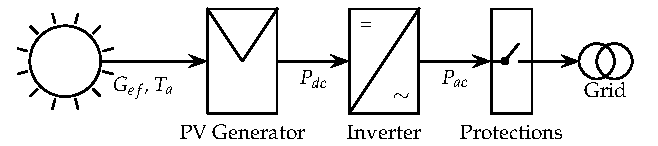
\includegraphics[width=.9\linewidth]{../figs/GCPVScheme.pdf}
\end{center}
\end{frame}

\section{Key concepts}
\label{sec:orgf7faae9}
\begin{frame}[label={sec:org255c1f3}]{Solar Radiation cannot be computed}
\begin{itemize}
\item Solar radiation reaching the earth surface is the result of \alert{complex interactions with the atmosphere}.
\item On-site measurements or satellite images are required for solar radiation estimation.
\end{itemize}
\begin{center}
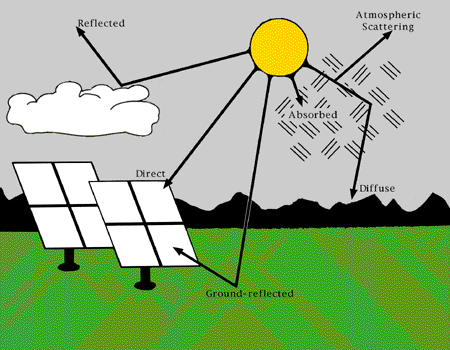
\includegraphics[height=0.5\textheight]{../figs/SolarRadiationComponents_NREL.png}
\end{center}
\end{frame}

\begin{frame}[label={sec:org46f3af5}]{Inclination Angle}
\begin{itemize}
\item PV generators have an \alert{inclination angle higher than zero} to maximize the performance.
\item The generator inclination angle depends on the latitude of the location and on the application\footnote{Rule of thumb: latitude minus 10º for a Grid Connected PV System; latitude plus 10º for a Standalone PV System.}.
\end{itemize}

\begin{center}
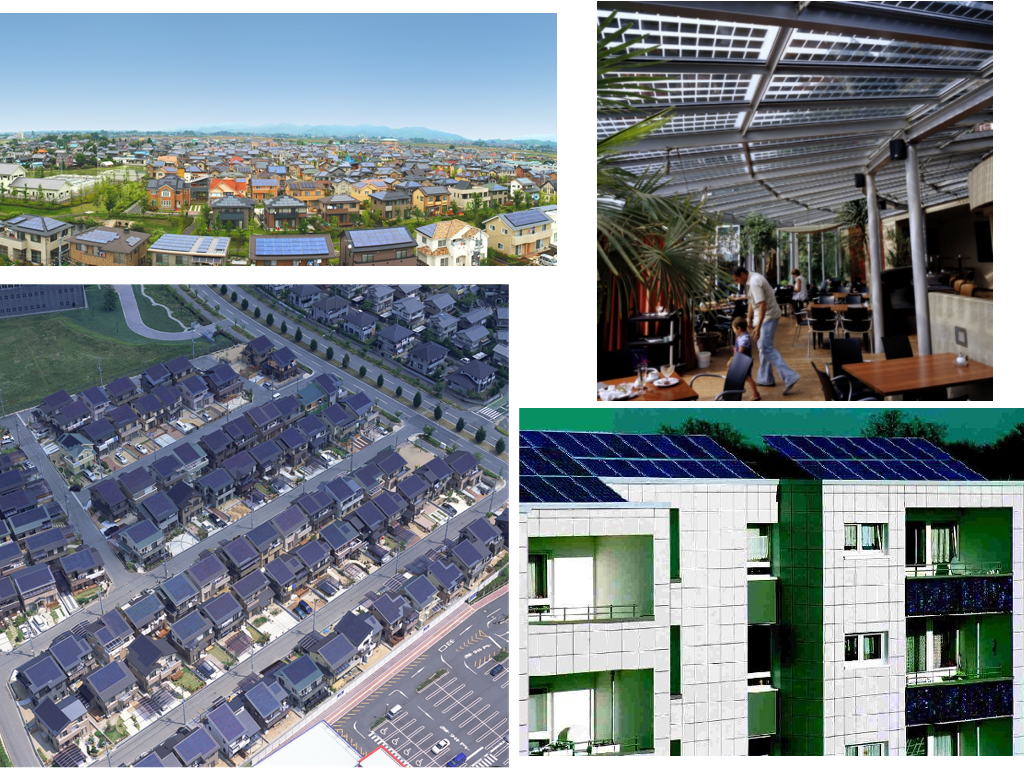
\includegraphics[height=0.5\textheight]{../figs/PVUrban.png}
\end{center}
\end{frame}

\begin{frame}[label={sec:org13a8db6}]{Solar Radiation Databases}
\begin{itemize}
\item Therefore, it is unfeasible to maintain a database of incident solar radiation.
\item Databases register solar radiation on the horizontal plane.
\item Estimation of the solar irradiation \alert{incident on the inclined plane} requires a transposition procedure.
\end{itemize}
\end{frame}


\begin{frame}[label={sec:org27dc8d3}]{From Horizontal to Inclined}
\begin{center}
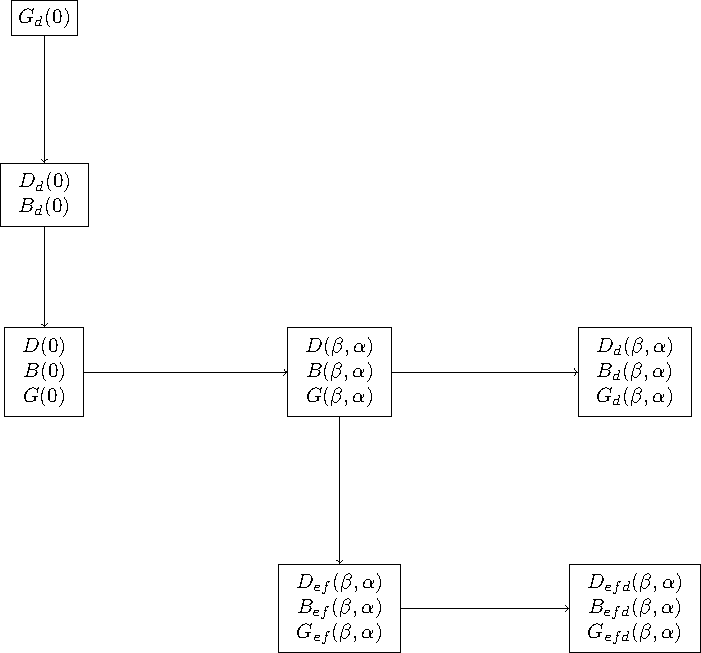
\includegraphics[width=.9\linewidth]{../figs/ProcedimientoCalculoRadiacionInclinada.pdf}
\end{center}
\end{frame}

\section{Definitions}
\label{sec:orgc3ae743}

\begin{frame}[label={sec:orge703812}]{Irradiance and Irradiation}
\begin{description}
\item[{Irradiance}] solar radiation \alert{power} received by a surface per unit area.
\begin{itemize}
\item Units: \(\si{\watt\per\meter\squared},\,\si{\kilo\watt\per\meter\squared}\)
\end{itemize}
\item[{Irradiation}] solar radiation \alert{energy} received by a surface per unit area.
\begin{itemize}
\item Units: \(\si{\watthour\per\meter\squared},\,\si{\kilo\watthour\per\meter\squared}\)
\item Hourly irradiation, Daily irradiation, Monthly irradiation \ldots{}
\end{itemize}
\end{description}
\end{frame}

\begin{frame}[label={sec:org5ccda1a}]{Extraterrestrial Solar Radiation}
\begin{itemize}
\item \(B_0\): Solar radiation energy/power at the top of the Earth's atmosphere on a surface perpendicular to the solar rays.
\item \(B_0 \simeq \SI{1367}{\watt\per\meter\squared}\) (Solar Constant)
\item \(B_0(0)\), extraterrestrial irradiance on a horizontal plane, can be computed by analytical means.
\begin{itemize}
\item Depends on the latitude, day of the year, hour of the day.
\end{itemize}
\end{itemize}
\end{frame}

\begin{frame}[label={sec:org56c8d69}]{Interaction with the Atmosphere}
Due to the interaction with the atmosphere, the extraterrestrial radiation is absorbed, reflected and scattered.

\begin{center}
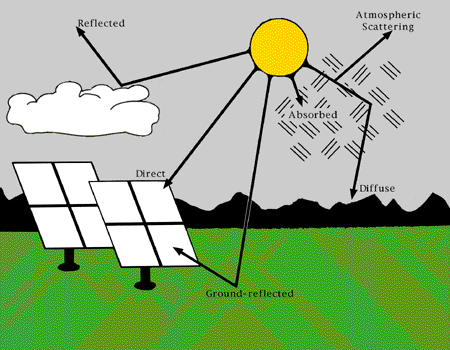
\includegraphics[height=0.5\textheight]{../figs/SolarRadiationComponents_NREL.png}
\end{center}
\end{frame}

\begin{frame}[label={sec:orgeee90ac}]{Diffuse, Beam, and Global}
\begin{itemize}
\item Solar radiation reaching the Earth surface is named \alert{global solar radiation}.
\item It is the result of three components:
\begin{itemize}
\item \alert{Beam Radiation}: solar radiation traveling on a straight line from the sun to the receiving surface.
\item \alert{Diffuse Radiation}: solar radiation scattered by the atmosphere. It is emitted from all directions of the sky.
\item \alert{Albedo or Reflected Radiation}: solar radiation reflected by the ground.
\end{itemize}
\end{itemize}

\begin{center}
\(G = B + D + R\)
\end{center}
\end{frame}

\begin{frame}[label={sec:org98e8507}]{Horizontal, Incident, Effective}
\begin{itemize}
\item \(G(0)\) \alert{Radiation on a Horizontal Plane} 
\begin{itemize}
\item Measurements from ground stations, or satellite images.
\end{itemize}
\item \(G(\alpha, \beta)\) \alert{Radiation incident on an Inclined Plane}
\begin{itemize}
\item Transposition from radiation on the horizontal plane.
\end{itemize}
\item \(G_{ef}(\alpha, \beta)\) \alert{Effective Radiation incident on a PV module}
\begin{itemize}
\item Reflectance and transmittance of the PV module depend on the angle of incidence.
\item Dirt losses.
\end{itemize}
\end{itemize}
\end{frame}
\end{document}